\chapter{Calico}
This section provides an overview of Calico and the functionality it provided before improvements began. There were four main components that made up the core functionality of Calico. The four components were:

\begin{itemize}\itemsep1pt

\item
\textbf{Canvas \& Grid}. 
Canvases provided users with a basic sketching area where all interaction would take place. The grid provided an easy way for designers to organize and arrange different canvases.

\item
\textbf{Scraps}.
Scraps provided groups of content that could be easily interacted with. In the section below, these interactions are discussed in further detail.

\item
\textbf{Gestures}.
Gestures allowed designers to provide an easily way to interact with the board by performing specific commands depending on the context they were in. The gestures in Calico were meant to copy normal whiteboard interactions, such as using a fist to erase sketches, and slashing through scraps to delete them.

\item
\textbf{Palettes}.
The palette in Calico provides designers with a temporary storage area for commonly used components.


\end{itemize}

In the following sections, each component will be explained in more detail.


\section{Canvas \& Grid}

Calico improves the design experience with four important features. These features are: a grid to manage multiple sketching canvases, scraps to represent different notations and improve manipulation of content, a palette to support reuse of sketched objects, and a gesture-based interaction paradigm for a fluid user experience.

% -----

% http://en.wikibooks.org/wiki/LaTeX/Floats,_Figures_and_Captions
\begin{figure}[htb]
  \centering
  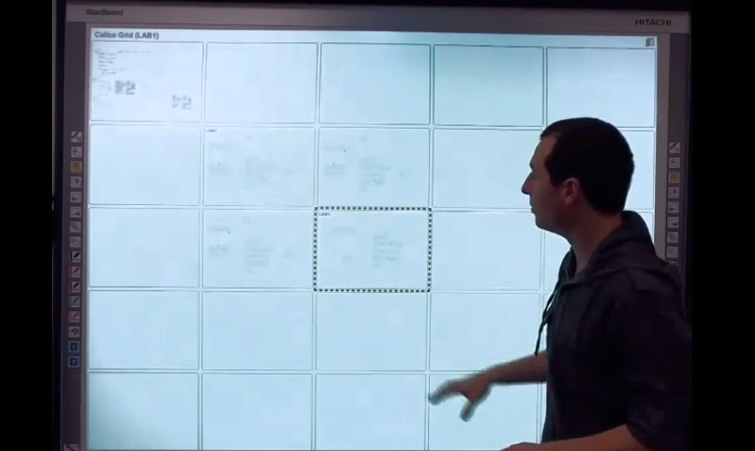
\includegraphics[width=0.8\textwidth]{grid.jpg}
  \caption{The grid view within Calico}
  \label{fig:grid}
\end{figure}
%The grid is the focal point of any session in Calico.
%It shows the various canvases that users may interact with in a given session.
%Users may perform various operations on canvases from the grid, such as duplicating or clearing individual cells.
%The grid also gives a clear overview of the designs that are happening in a session.

% ANDRE:
% Grid is an organizing space for sketches
% Move cells around
% build a history by making copies of the cells
% you can move select cells to different locations
% why does the grid exist?
% why it mentally does for the user
% why the features are what they are
Designers not only need to keep track of their work, but they also need to constantly shift focus in their designs.
The grid acts as an organizational tool for the sketches, and also allows designers to easily shift focus. [See Figure \ref{fig:grid}]
The grid organizes sketching areas in a row-column fashion, much like a spreadsheet organizes data. 
In Calico, ``canvases'' are used instead of cells which are used in a spreadsheet.
From the grid, designers can easily drag canvases and reposition them in different locations. This allows designers to logically organize their designs, as they can separate different designs (even completely different systems) from each other so that there is no confusion. 
The grid also allows designers to create a history of their design process by allowing them to create copies of existing canvases, so that their original design can be quickly compared with a new branch of thought. Each grid ``cell'' consists of a single sketching canvas. Users are able to freely sketch within each canvas, and canvases are kept separate from other canvases, so that designers can work uninterrupted. Each of these canvases can contain sketches, writings, or anything that the designer desires. 


% TABS
\begin{figure}[h]
  \centering
  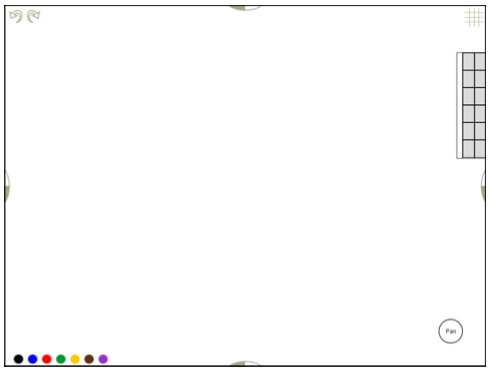
\includegraphics[width=0.6\textwidth]{blank_canvas.png}
  \caption{The default canvas view in Calico}
  \label{fig:canvas}
\end{figure}
Standard whiteboards do not easily allow designers to shift their focus quickly. This means that it is difficult for designers to create branches of their designs. If a designer wants to create a branch, they first need to duplicate their entire design elsewhere before they can erase it. The alternative would be to branch using the existing design, which would essentially destroy the previous design. Neither of these options are desirable as they lead to less design exploration -- hindering the design process. To remedy this problem, Calico has four gray tabs located on all edges of the sketching area. [See Figure \ref{fig:canvas}]. By clicking any one of the gray tabs, the entire contents of the current canvas is copied to the relevant adjacent canvas, and focus is then shifted to this newly created canvas. This allows designers to further explore an different design idea, but still allows them to revert to a previous state of their design. By repeatedly using tabs to create new design branches, a designer can develop a history of the evolution of their design. The designer essentially creates a ``filmstrip'' of activity that can serve as a timeline for the design\cite{filmstrip}. Using Calico's grid system, designers can arrange various canvases into groups that can be used to represent different concerns, or even separate ``old'' designs from newer ones.



\section{Scraps}

\begin{figure}[htb]
  \centering
  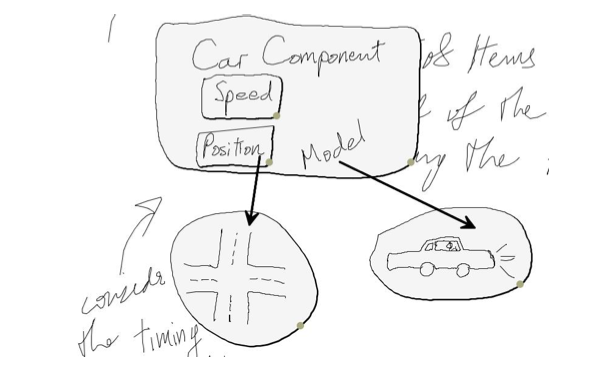
\includegraphics[width=0.8\textwidth]{scraps.png}
  \caption{Scraps (gray background) within Calico}
  \label{fig:scraps}
\end{figure}

Scraps in Calico can be thought of as ``scraps of paper'' that one would place on a desk or on a white board.
Scraps keep their shape -- whatever the designer draws, this shape will be kept throughout the design phase.
However, scraps are manipulatable in many different ways -- they are stackable, removable, relatable, movable. 
In the original version of Calico, all scraps have a ``dot'' that acts as a menu where various actions can be performed on the scrap itself.
Our goal is to be able to interact with the designers so that they are able to manipulate the objects, but we do not want to be intrusive in the way a formal design tool would be.

We created scraps as the answer to allowing the content of a sketched design to become ``active'', while still allowing the designer to be completely free in their design and still able to manipulate their sketches.
Designers tend to use many different notations when they are designing, and we want designers to be able to sketch in the notations that they are most comfortable with, but we also want to be able to work with their designs.
The key is that we leave them in the same shape they were in when they were drawn, but that they become ``active''. 
Anything drawn on top of that scrap automatically comes associated with the original scrap.
Designers can relate scraps with each other simply by drawing a line from one to the other, which would be converted to a directional arrow, linking the two scraps with each other.



\section{Gestures}
Many of the actions that Calico is designed to support require fluidity and speed of sketching. Calico should be as unobtrusive as possible to a designer. In order to be as unobtrusive as possible, common operations (such as erasing, or moving items) should be very easy to perform. The fluidity and flow of the design process needs to be maintained, and objects need to be created as the designer wants. The cost of making design changes has to be low \cite{design_fluidity}, so that designers are not impeded by the design software.

Menu-driven interaction greatly impedes the fluidity of the design process. Allowing all operations to be accessible using gestures would require many complex gestures that would be very difficult for users to remember or perform. In an effort to reduce this effect, Calico uses mixed-mode interaction: commonly performed operations are available using gestures, while complex and less used operations are available via an easily accessible menu. This reduces the number of gestures (and complexity of gestures), while still allowing the design process to be fluid.

Gestures in Calico are context-sensitive. Sketching can have different meanings depending on various parameters. Scraps could be easily removed without requiring a break in the user's thought process by performing a ``slash'' gesture across a scrap, which would immediately erase the scrap and it's contents.
As a diagramming tool, users were constantly linking scraps to show inheritance, abstraction, etc.
Calico also allows users to draw a line from one scrap to another scrap, and this will be automatically transformed into a directed arrow, which would link the two scraps.
Once two scraps are linked, the arrow is then anchored to them, and would follow the scrap whenever it is moved on screen.
Another gesture that was added was the ability to enlarge a scrap by drawing a ``blister'' or bubble on the edge of the scrap.
By drawing this extra bubble, the scrap area would be enlarged to equal the size of the bubble that was just drawn. These actions together create a powerful interaction method that allows the user to create and manipulate scraps, draw arrows to link scraps together, and to navigate the Calico interface easily. 

% Nick
% \begin{itemize}
%   \item The first item
%   \item The second item
%   \item The third etc \ldots
% \end{itemize}

%Scraps can be easily relocated to different parts of the screen, or even other canvases.
%Scraps can be stacked on top of each other and then treated as a unit or group.
%By treating scraps as if they were pieces of paper, we [make it easy to understand the manipulation], as designers can easily relate Calico to their current design 

\section{Palette}
The palette in Calico provides users with a ``drawer'' that can easily be used to store commonly used shapes and artifacts.
\begin{figure}[htb]
  \centering
  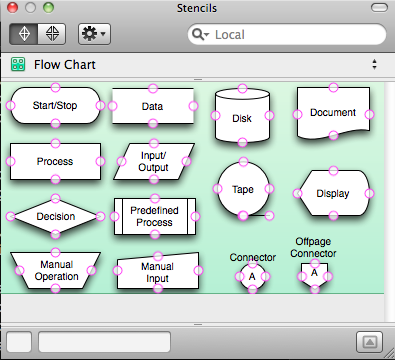
\includegraphics[width=0.5\textwidth]{palette.png}
  \caption{A container for commonly used components being used in Omnigraffle}
  \label{fig:palette_omnigraffle}
\end{figure}
The concept of a palette is something that can be seen in many current design programs. One example of this would be in Omnigraffle\cite{todo}. As shown in Figure \ref{fig:palette_omnigraffle}, the palette provides easy access to components that are commonly used during the design process. However, in most design tools this palette is populated with a predefined set of components, and this list cannot be modified by the designer. Due to the fact that Calico was designed to support the informal design process, it was decided that components in the palette should be determined by the designer. In Calico, the palette begins as a blank storage area that can be populated with content created by the designer, which allows for the reuse of sketched elements. 

The palette was designed to store scraps. To place a scrap into the palette, a designer simply need to drag the scrap into one of the available storage slots. The scrap (and any children of the scrap) would then be stored into the palette. The palette in Calico acted as a global storage area that was available on all canvases. This enabled designers to easily reuse components on different branches of design, or on completely different design sessions.  




% NICK
% Palettes are not new, but their typical incarnation in drawing programs is to include a prepopulated set of figures that are not configurable beyond changing the entire set. In design, however, it is not uncommon that a sponta- neous notational convention emerges that does not necessarily adhere to any pre-existing or fixed set of figures. Calico’s palette, thus, starts empty, and is filled with content by the designer, enabling the reuse of sketched elements. This allows a temporary vocabulary to be created and leveraged within a design session (as exemplified by the impromptu notations in Figure 10, as further described in Section 6).
% The palette leverages scraps for this purpose. Designers can store a scrap simply by dragging it into the palette on the side of Calico’s canvas (visible on the right-hand side of Figure 3). The palette has a number of cells, each of which may hold one or more scraps. By dragging from a palette cell onto the canvas, any scraps inside that cell are copied to the canvas at the position of the stylus. Once populated, the user can rapidly create variations of a design simply by dragging key scraps from the palette. Note that the palette serves as a global clipboard; scraps can be stored and reused from any canvas.